\documentclass[a4paper, twocolumn, oneside, 10pt]{article}

\usepackage{xstring}
\usepackage{xparse}
\usepackage{blindtext}
\usepackage{amsfonts}
\usepackage{amsmath}
\usepackage{amssymb}
\usepackage{tikz}
\usepackage{siunitx}
\usepackage{longtable}
\usetikzlibrary{arrows.meta}
\usepackage{algorithm}
\usepackage{algpseudocode}
\usepackage[margin=30mm]{geometry}
\usepackage[backend=bibtex,style=ieee]{biblatex}
\usepackage{pgfplots}
\usepackage{todonotes}
\usepackage[labelfont=bf]{caption}

\usepackage[barriers=false]{acro}
\NewDocumentCommand\acrodef{mO{#1}mG{}}{\DeclareAcronym{#1}{short={#2}, long={#3}, #4}}
\NewDocumentCommand\acused{m}{\acuse{#1}}
\usepackage[hidelinks]{hyperref}
\usepackage[capitalise]{cleveref}
\crefname{section}{section}{sections}
\crefname{figure}{figure}{figures}
\crefname{table}{table}{tables}
\crefname{equation}{equation}{equations}
\crefname{algorithm}{algorithm}{algorithms}
\Crefname{section}{Section}{Sections}
\Crefname{figure}{Figure}{Figures}
\Crefname{table}{Table}{Tables}
\Crefname{equation}{Equation}{Equations}
\Crefname{listing}{Listing}{Listings}
\crefname{algorithm}{Algorithm}{Algorithms}
\def\figname{\csname cref@figure@name\endcsname\xspace}
\def\tabname{\csname cref@table@name\endcsname\xspace}
\def\secname{\csname cref@section@name\endcsname\xspace}
\def\eqname{\csname cref@equation@name\endcsname\xspace}
\def\eqpname{\csname cref@equation@name@plural\endcsname\xspace}
\def\eqname{\csname cref@listing@name\endcsname\xspace}
\def\eqname{\csname cref@listing@name@plural\endcsname\xspace}

\acrodef{CMKP}{Clustered Multidimensional Knapsack Problem}
\acrodef{ILP}{Integer Linear Problem}
\acrodef{LP}{Linear Problem}
\acrodef{MKP}{Multidimensional Knapsak Problem}
\acrodef{MIP}{Mixed Integer Programming}

\title{The \ac{CMKP}}
\author{E.Brambilla, M.Cherubini, S.Fontana, C.Metelli, J.Tedeschi}
\date{\today}
\addbibresource{bibliography.bib}

\begin{document}
\twocolumn[
  \begin{@twocolumnfalse}
    \maketitle
    \begin{abstract}
      This project aims to provide an efficient heuristic method to approach the \ac{CMKP} capable of producing good feasible solutions in a limited-time environment. This project will be evaluated against the solutions of benchmark instances found by the Gurobi\cite{gurobi} solver. The goal of this project is to deonstrate the above-mentioned heuristic can deliver close --- or better --- solutions to the plain solver results in a reduced amount of time.
    \end{abstract}
    \vspace{5mm}
  \end{@twocolumnfalse}
]

\section{Introduction}\label{sec:problem}
A construction company must plan its next investments. Its core business consists of buying lots of land, constructing new buildings, and making a profit by selling them. 
Each lot of land can be allocated for the construction of one or more buildings in different combinations and, regardless of the chosen configuration, certain resources cannot exceed a fixed value for each individual lot. 
Also, some global resources that take into account all buildings built by the company must not exceed a fixed quantity. From now on we will refer to those quantities
as resources. 
The goal of the construction company is to maximize the total profit expected from the sale of
the new buildings minus the cost of purchasing the lots of land chosen as construction sites.
Given \(\bar{n} \in \mathbb{N}^+\), let \(\mathbf{I} = \{ 1, \ldots , \bar{n} \}\) be the set of available lots of land and let \(q_i \in \mathbb{N}\)  be the cost of purchasing lot \( i \in \mathbf{I}\). 
For each lot, \(i \in \mathbf{I}\), let \(C_i = \{ 1, \ldots , c_i \}\) be the set of buildings that the construction company may build inside lot i and let \(p_{ij} \in \mathbb{N} (i \in \mathbf{I}, j \in C_i)\) be its profit. 
Also, for each lot of land \(i \in \mathbf{I}\), let \(R_i\) be the set of local resources that must not exceed a given amount and let \(b_{ir} \in \mathbb{N}\) be the maximum amount of resource \(r \in R_i\) that can be used. Finally, let \(\mathbf{R}\) be the set of global resources and, for each \(r \in \mathbf{R} \), let \(b_r \in \mathbb{N} \) be the total value that cannot be exceeded. 
Each building \(j \in C_i, i \in \mathbf{I}\) consumes an amount of resource \(r \in \mathbf{R} \cup R_i\) equal to \(a^r_{ij} \in \mathbb{N}\).

\subsection{ILP Modelization}
The analyzed \ac{ILP} follows the proposed formulation\cite{assignment} without any additional constraints. The formulation is reported below.

Given the sets and parameters defined in \cref{sec:problem}, the \ac{ILP} formulation is the following:
\begin{align}
	&\max \sum_{i \in \mathbf{I}, j \in C_i} p_{ij}x_{ij} - \sum_{i\in\mathbf{I}} q_{i}y_i \label{eqn:ilp-obj}\\
	\omit s.t. \notag & \\
	&\sum_{i \in \mathbf{I}, j \in C_i} a^r_{ij}x_{ij} \leq b_r \ \quad \forall r \in \mathbf{R} \label{eqn:ilp-global-cap}\\
	&\sum_{i \in \mathbf{I}} a^r_{ij}x_{ij} \leq b_{ir} \quad  \forall i \in \mathbf{I}, \forall r \in R_i \label{eqn:ilp-local-cap} \\
	&x_{ij} \leq y_i \quad \forall i \in \mathbf{I}, \forall j \in C_i, \label{eqn:ilp-building-selection}\\
	&x_{ij}, y_i \in \big\{0, 1\big\} \quad \forall i \in \mathbf{I}, \forall j \in C_i \label{eqn:ilp-binary}
\end{align}
where \(x_{ij}\) and \(y_i\) are binary selection variables as per \cref{eqn:ilp-binary}.
The goal of \cref{eqn:ilp-global-cap} is to impose a limit, over all the selected buildings, to the global capacities. Similarly, \cref{eqn:ilp-local-cap} aims to limit local-capacities for same-lot buildings.
The constraint \cref{eqn:ilp-building-selection} ensures buildings for a lot \(i \in \mathbf{I}\) can be selected iff.\ the lot \(i\) itself is selected.
This is the most stringent constraint formulation which also includes the biggest number of constraints to be put in the problem. Alternatively, the constraint \(\sum_{j \in C_i} x_{ij} \leq |C_i|y_i \quad \forall i \in \mathbf{I}\) could be used resulting in less stringent --- thus less useful --- \ac{ILP} formulation.

\section{Heuristic algorithm}\label{sec:heuristic}
The heuristic model chosen for the development of this project is the Kernel Search\cite{angelelli2010kernel}. This heuristic approach has been proved to be very efficient in the \ac{MKP} class which is noticeably similar to the \ac{CMKP}. Particularly, we can define the \ac{MKP} as a relaxed version of the \ac{CMKP} by removing the lot selection constraint (\cref{eqn:ilp-building-selection}) and by forcing \(y_i = 1\). By this assumption, the cost of lot purchase can be removed from the objective function (\cref{eqn:ilp-obj}) as it will become a constant and the whole problem can be seen as a \ac{MKP} with the addition of local resources.

It is non trivial though to find an efficient ordering method for the variables in the problem, given the clustered nature of the buildings. More precisely, the cost of the lot cannot be included in a single variable for ordering. Also, the cost of the chosen lot will be partitioned over every selected building inside it, reducing its influence with the number of chosen variables \(x_{ij}\). Because of this non-linearity in the lot cost partitioning, a globally valid sorting methodology has not been found.

\subsection{Sorting Method}

\begin{figure}
	\centering
	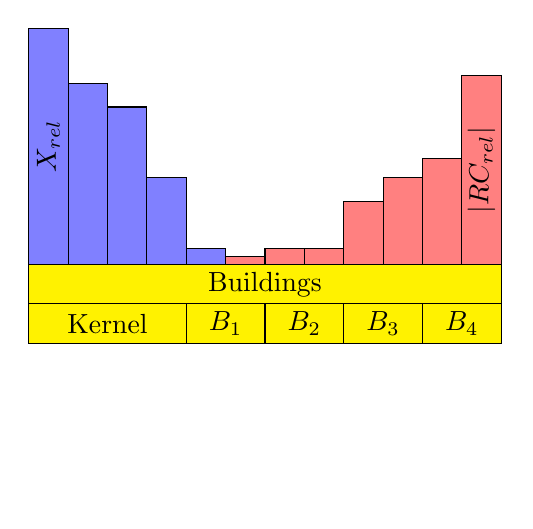
\begin{tikzpicture}
%		\draw[help lines] (0,0) grid (6,4);
		\fill[white] (0, -2) rectangle ++(6,0.5);		
		\draw[fill=yellow] (0, 0.5) rectangle ++(6,0.5) node[pos=.5] {Buildings};		
		\draw[fill=yellow] (0, 0) rectangle ++(2,0.5) node[pos=.5] {Kernel};
		\draw[fill=yellow] (2, 0) rectangle ++(1,0.5) node[pos=.5] {\(B_1\)};
		\draw[fill=yellow] (3, 0) rectangle ++(1,0.5) node[pos=.5] {\(B_2\)};
		\draw[fill=yellow] (4, 0) rectangle ++(1,0.5) node[pos=.5] {\(B_3\)};		\draw[fill=yellow] (5, 0) rectangle ++(1,0.5) node[pos=.5] {\(B_4\)};
		
		\draw[fill=blue!50] (0, 1) rectangle ++(0.5,3) node[pos=.5, rotate=90] {\(X_{rel}\)};
		\draw[fill=blue!50] (0.5, 1) rectangle ++(0.5,2.3);
		\draw[fill=blue!50] (1, 1) rectangle ++(0.5,2);
		\draw[fill=blue!50] (1.5, 1) rectangle ++(0.5,1.1);
		\draw[fill=blue!50] (2, 1) rectangle ++(0.5,0.2);
		
		\draw[fill=red!50] (2.5, 1) rectangle ++(0.5,0.1);
		\draw[fill=red!50] (3, 1) rectangle ++(0.5,0.2);
		\draw[fill=red!50] (3.5, 1) rectangle ++(0.5,0.2);
		\draw[fill=red!50] (4, 1) rectangle ++(0.5,0.8);
		\draw[fill=red!50] (4.5, 1) rectangle ++(0.5,1.1);
		\draw[fill=red!50] (5, 1) rectangle ++(0.5,1.35);
		\draw[fill=red!50] (5.5, 1) rectangle ++(0.5,2.4) node[pos=.5, rotate=90] {\(|RC_{rel}|\)};
	\end{tikzpicture}
	\caption{Standard sorting method for kernel search\cite{angelelli2010kernel}: Selection variables are sorted globally by their relaxed value (decreasing) at optimum and by their absolute reduced costs (increasing).}\label{fig:kernel-std-sort}
\end{figure}

\begin{figure}
	\centering
	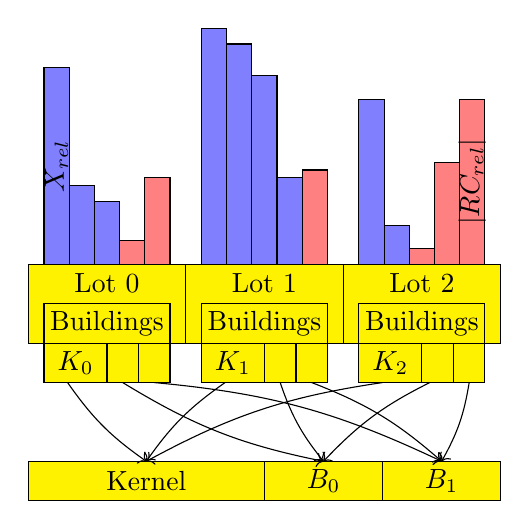
\begin{tikzpicture}
		\draw[fill=yellow] (0, 0) rectangle ++(2,1) node[pos=.5, yshift=7.5] {Lot 0};
		\draw[fill=yellow] (2, 0) rectangle ++(2,1) node[pos=.5, yshift=7.5] {Lot 1};
		\draw[fill=yellow] (4, 0) rectangle ++(2,1) node[pos=.5, yshift=7.5] {Lot 2};
		\draw[fill=yellow] (0.2, 0) rectangle ++(1.6,0.5) node[pos=.5] {Buildings};
		\draw[fill=yellow] (2.2, 0) rectangle ++(1.6,0.5) node[pos=.5] {Buildings};
		\draw[fill=yellow] (4.2, 0) rectangle ++(1.6,0.5) node[pos=.5] {Buildings};
		
		\draw[fill=blue!50] (0.2, 1) rectangle ++(0.32,2.5) node[pos=.5, rotate=90] {\(X_{rel}\)};
		\draw[fill=blue!50] (0.52, 1) rectangle ++(0.32,1);
		\draw[fill=blue!50] (0.84, 1) rectangle ++(0.32,0.8);
		\draw[fill=red!50] (1.16, 1) rectangle ++(0.32,0.3);
		\draw[fill=red!50] (1.48, 1) rectangle ++(0.32,1.1);
		
		\draw[fill=blue!50] (2.2, 1) rectangle ++(0.32,3);
		\draw[fill=blue!50] (2.52, 1) rectangle ++(0.32,2.8);
		\draw[fill=blue!50] (2.84, 1) rectangle ++(0.32,2.4);
		\draw[fill=blue!50] (3.16, 1) rectangle ++(0.32,1.1);
		\draw[fill=red!50] (3.48, 1) rectangle ++(0.32,1.2);
		
		\draw[fill=blue!50] (4.2, 1) rectangle ++(0.32,2.1);
		\draw[fill=blue!50] (4.52, 1) rectangle ++(0.32,0.5);
		\draw[fill=red!50] (4.84, 1) rectangle ++(0.32,0.2);
		\draw[fill=red!50] (5.16, 1) rectangle ++(0.32,1.3);
		\draw[fill=red!50] (5.48, 1) rectangle ++(0.32,2.1) node[pos=.5, rotate=90] {\(|RC_{rel}|\)};
		
		\draw[fill=yellow] (0.2, -0.5) rectangle ++(0.8,0.5) node[pos=.5] {\(K_0\)};
		\draw[fill=yellow] (1, -0.5) rectangle ++(0.4,0.5);
		\draw[fill=yellow] (1.4, -0.5) rectangle ++(0.4,0.5);
		
		\draw[fill=yellow] (2.2, -0.5) rectangle ++(0.8,0.5) node[pos=.5] {\(K_1\)};
		\draw[fill=yellow] (3, -0.5) rectangle ++(0.4,0.5);
		\draw[fill=yellow] (3.4, -0.5) rectangle ++(0.4,0.5);
		
		\draw[fill=yellow] (4.2, -0.5) rectangle ++(0.8,0.5) node[pos=.5] {\(K_2\)};
		\draw[fill=yellow] (5, -0.5) rectangle ++(0.4,0.5);
		\draw[fill=yellow] (5.4, -0.5) rectangle ++(0.4,0.5);
		
		\draw[fill=yellow] (0, -2) rectangle ++(3,0.5) node[pos=.5] {Kernel};
		\draw[fill=yellow] (3, -2) rectangle ++(1.5,0.5) node[pos=.5] {\(B_0\)};
		\draw[fill=yellow] (4.5, -2) rectangle ++(1.5,0.5) node[pos=.5] {\(B_1\)};
		
		\draw[->] (0.5, -0.5) to [bend right=10] (1.5, -1.5);
		\draw[->] (2.5, -0.5) to [bend right=10] (1.5, -1.5);
		\draw[->] (4.5, -0.5) to [bend right=10] (1.5, -1.5);
		\draw[->] (1.2, -0.5) to [bend right=10] (3.75, -1.5);
		\draw[->] (3.2, -0.5) to [bend right=10] (3.75, -1.5);
		\draw[->] (5.1, -0.5) to [bend right=10] (3.75, -1.5);
		\draw[->] (1.6, -0.5) to [bend left=10] (5.25, -1.5);
		\draw[->] (3.6, -0.5) to [bend left=10] (5.25, -1.5);
		\draw[->] (5.6, -0.5) to [bend left=10] (5.25, -1.5);
	\end{tikzpicture}
	\caption{Sorting method utilized for this project}\label{fig:kernel-cust-sort}
\end{figure}

Instead of a global sorting method as depicted in \cref{fig:kernel-std-sort}, where the \ac{LP} relaxation is resolved and the variables are then ordered by decreasing relaxed value and by increasing reduced cost, a different approach has been chosen: the kernel and the buckets are constructed by selecting sub-kernels and sub-buckets from each different lot. Lots selection is then left for decision to Gurobi during the solution of the sub problem. We then treat each lot buildings as a single instance to be ordered through the method depicted in \cref{fig:kernel-std-sort}. A visual representation of this sorting method is depicted in \cref{fig:kernel-cust-sort}. 

Given a set of lots \(\mathbf{I} = \big\{1\ldots\bar{n}\}\) each containing \(n_i\) buildings, the list of buildings in each lot \(\mathbf{C}\), and the sizes of the sub-kernels and sub-buckets, the sorting algorithm works as described in \cref{alg:kernel-sort-cust}.

\begin{algorithm}
	\caption{Kernel Search sorting algorithm used}\label{alg:kernel-sort-cust}
	\begin{algorithmic}
		\Function{SortBuildings}{$\mathbf{I}$, $\mathbf{C}$, $K_{size}$, $B_{size}$}
			\State $rel \gets$ \Call{ResolveLPRelaxation}{$\mathbf{I}$}
			\State $K \gets \emptyset$%
			\State $B \gets \emptyset$%
			\ForAll{$l \in \mathbf{I}$}
				\State \Call{SortLot}{$l$, $rel$}%
				\State $K \gets K \cup $\Call{GetBlds}{$l$, $0$, $|C_i|\cdot K_{size}$}
				\State $len \gets K_{size}$%
				\State $i \gets 0$%
				\While{$len \leq |C_l|$}
					\State $B[i] = B[i] \cup$\Call{GetBlds}{$l$, $len$, $|C_i|\cdot B_{size}$}
					\State $len \gets len + B_{size}$%
					\State $i \gets i + 1$%
				\EndWhile%
			\EndFor%
			\State \Return{K, B}%
		\EndFunction%
	\end{algorithmic}
\end{algorithm}

The concept behind \cref{alg:kernel-sort-cust} is the following: after having solved the \ac{LP} relaxation of the main problem, each lot can be seen as a \ac{MKP} with additional global constraints. Because of this, each lot of buildings can now be sorted as if it was a simpler problem as described by E.Angelelli et al.\cite{angelelli2010kernel} by sorting the variables by value and reduced costs. 
We can then identify a kernel \(K_l\) for each lot \(l \in \textbf{I}\) as the \(K_{size}\) most promising buildings for the lot. We define the problem's kernel \(K\) as the union of each sub-kernel \(K_l\). Formally: \[K = \bigcup_{l \in \mathbf{I}} K_l\]

During the kernel search iteration procedure, multiple sub-problems have to be solved with the addition of new variables added to the problem in the form of buckets. We decided to iterate over each bucket of fixed size \(|\mathbf{I}| \cdot B_{size}\) composed similarly to the kernel \(K\) as following: \[B_i = \bigcup_{l \in \mathbf{I}} B_{li}\]

Each time a new bucket is added, a new constraint, defined in \cref{eqn:must-select} is added to the problem stating that at least one building of the newly added bucket \(B_i\) has to be chosen in a new incumbent solution for the current iteration. Also, once a new incumbent solution has been found, a new cutoff constraint must be added excluding all solutions with objective value lower than or equal to the newly found incumbent solution.

\begin{equation}\label{eqn:must-select}
	\sum_{i \in \mathbf{I}, j \in C_i : x_{ij} \in B_i} x_{ij} \geq 1 
\end{equation}

On new solutions, the variables chosen in the last bucket are then included in the kernel set \(K\).

Ideally, non-useful lots are going to be excluded in the first few iterations and thus are not going to provide kernel set additions reducing the number of variables in the problem. Contrarily, useful lots may be excluded in the beginning, limiting their ability to provide variables and so to be selected again. This problem can be managed by applying the solution defined in \cref{sec:lot-iteration}.

\subsection{Lot iteration}\label{sec:lot-iteration}
In order not to reject useful lots and to allow for faster sub-problems, we managed to implement a lot-based iteration step. The algorithm becomes effectively a kernel search made amongst buildings inside a kernel search made amongst lots.

This method allows to reiterate over buckets inside the most promising lots and still add new variables to the problem.

The conceptual algorithm is reported in \cref{alg:lot-iter}. The idea of the algorithm is to reduce the initial number of variables in the kernel and the buckets by forcing part of the \(y_i\) variables to zero. The sub-problem is solved with the kernel search heuristic discussed in \cref{sec:heuristic}. After this preliminary solution, Another set of \(y_i\) variables is allowed to be chosen and the iteration is repeated by keeping the initial kernel. This allows to reintroduce discarded bucket variables from the previous iteration in the previous lot set and still extend the kernel set with the new lot's variables. Lot sorting is discussed in \cref{sec:lot-iteration-ordering}

\begin{algorithm}
	\caption{Lot iteration algorithm}\label{alg:lot-iter}
	\begin{algorithmic}
		\Function{IterateLots}{$\mathbf{I}$, $\mathbf{C}$, $K_{size}$, $B_{size}$}
		\State $cur \gets \emptyset$
		\State $sol \gets \emptyset$
		\State \Call{SortLots}{$\mathbf{I}$, $\mathbf{C}$, $sol$}
		\While{$I \neq \emptyset$}
			\State $cur \gets cur \cup $ \Call{GetFirstN}{$I$}
			\State $I \gets I - cur$
			\State $sol \gets $\Call{BKS\footnotemark}{$cur$, $\mathbf{C}$, $K_{size}$, $B_{size}$, $sol$}
		\EndWhile
		\State \Return $sol$
		\EndFunction
	\end{algorithmic}
\end{algorithm}
\footnotetext{BuildingKernelSearch}

\subsubsection{Lot ordering}\label{sec:lot-iteration-ordering}
Given a set of lots \(\mathbf{I}\) and the current incumbent solution \(\bar{S}\), for each lot \(l \in \mathbf{I}: \bar{S}(y_l) = 0\) we define the \(l\)-relaxation over the solution \(\bar{S}\) as a \ac{MKP} with the buildings of lot \(l\) constraining all its local capacity constraints and all global constraints in a reduced form \(\bar{R}\) defined in \cref{eqn:reduced-form}. 

\begin{equation}\label{eqn:reduced-form}
	\bar{R}_i = R_i - \sum_{j \in C_l} a^r_{lj}x_{lj}
\end{equation}

The \ac{LP} relaxation optimal objective value is then taken as the metric for the sorting of the lots.

\subsubsection{Lot Filtering}

One downside of the Kernel Search approach is that the kernel keeps getting bigger by adding to it the selected variables of the bucket in a given iteration. This behavior causes the solution time for the \(i\)-th iteration \ac{MIP} to increase steadily, limiting the quality of later solutions.

We tried to patch this behavior by implementing an exclusion policy alongside the previously mentioned lot iteration at \cref{sec:lot-iteration}. Implementing a slight modification on \cref{alg:lot-iter}, represented in \cref{alg:lot-iter-filter}, we defined such elimination-rule to be executed after each lot-limited subproblem. 
\cref{alg:lot-iter-filter}'s idea is to remove not selected lots from the incumbent solution --- and consequently their buildings from the kernel --- in order to limit the possible choices during the next iteration.

\begin{algorithm}
	\caption{Lot iteration algorithm with filtering}\label{alg:lot-iter-filter}
	\begin{algorithmic}
		\Function{IterateLotsFlt}{$\mathbf{I}$, $\mathbf{C}$, $K_{size}$, $B_{size}$}
		\State $cur \gets \emptyset$
		\State $avail \gets \mathbf{I}$
		\State $excluded \gets \emptyset$
		\State $sol \gets \emptyset$

		\While{$avail \neq \emptyset$}
			\State \Call{SortLots}{$avail$, $\mathbf{C}$, $sol$}

			\State $cur \gets cur \cup $ \Call{GetFirstN}{$avail$}
			\State $avail \gets avail - cur$
			\State $sol \gets $\Call{BKS}{$cur$, $\mathbf{C}$, $K_{size}$, $B_{size}$, $sol$}
			\State $avail \gets avail \cup excluded$

			\State $excluded \gets \{l \in cur : sol(y_l) = 0\}$
			\State $cur \gets cur - excluded$
		\EndWhile
		\State \Return $sol$		
		\EndFunction
	\end{algorithmic}
\end{algorithm}

\begin{figure}
	\centering
	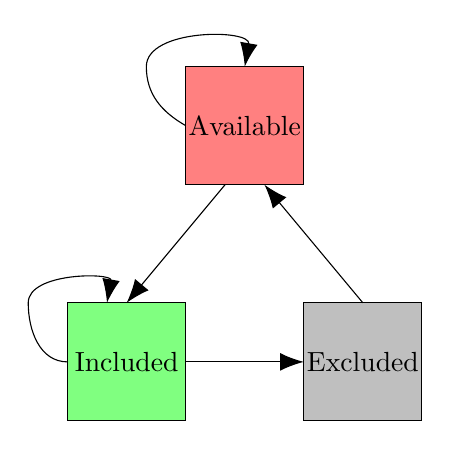
\begin{tikzpicture}
		\draw[fill=green!50] (0, 0) rectangle ++(1.5, 1.5) node[pos=.5] {Included};
		\draw[fill=gray!50] (3, 0) rectangle ++(1.5, 1.5) node[pos=.5] {Excluded};
		\draw[fill=red!50] (1.5, 3) rectangle ++(1.5, 1.5) node[pos=.5] {Available};

		\draw[-{Latex[length=3mm]}] (1.5, 0.75) to (3, 0.75);
		\draw[-{Latex[length=3mm]}] (2, 3) to (0.75, 1.5);
		\draw[-{Latex[length=3mm]}] (3.75, 1.5) to (2.5, 3);
		\draw[-{Latex[length=3mm]}] (0, 0.75) to[out=180, in=-90] (-0.5, 1.5) to[out=90,in=80] (0.5, 1.5);
		\draw[-{Latex[length=3mm]}] (1.5, 3.75) to[out=150, in=-90] (1, 4.5) to[out=90,in=80] (2.25, 4.5);

	\end{tikzpicture}
	\caption{Lot state management diagram. Each transition is performed after an iteration.}\label{fig:lot-state-mgmt}
\end{figure}

The removed lots are going to be reintroduced in later iterations only if the lot metric (defined as per \cref{sec:lot-iteration-ordering}), recomputed at each iteration based on the newly found incumbent solution, finds the lot one of the most valuable. This behavior ensures the previously discarded lot to be added to the solution only if really required.

Lot state management has to keep count of the lots discarded in the previous iteration in order to avoid looping as described by \cref{fig:lot-state-mgmt} resembling the base feature described in the ``Tabu Search'' algorithm\cite{glover1990tabu}. When started, the algorithm will set the state of each lot either ``Included'' in the next iteration or ``Available''. Loop prevention is archived in case of an included lot not being selected after the iteration by passing it into an excluded state.
Exclusion can last only one iteration, with excluded lots becoming available the next round.
More precisely, if this solution is not applied, removed lots can be inserted into the next iteration resulting in a similar solution which will exclude the lots again, looping forever without increasing the quality of the solution. 
Thus the chosen implementation: at the beginning a set of lots is assigned to the ``Available'' state. Each iteration starts with the sorting of all the ``Available'' lots and the insertion of the first \(N\) into the current lot list used for the Kernel Search process (reduced lot kernel search). Once the iteration is concluded, excluded lots are set to the ``Excluded'' state and previously excluded lots are reintegrated into the ``Available'' list. 
This procedure \textit{de-facto} eliminates two-iteration loops but won't prevent higher order ones. Conceptually the probability of a three(or more)-iteration loop is very low because ideally each iteration will produce a new incumbent solution given by the addition of new lots into the variable space.


\subsubsection{Kernel Filtering}\label{sec:kernel-filtering}

\begin{figure}
	\centering
	\resizebox{\columnwidth}{!}{
		\begin{tikzpicture}
			\begin{axis}[
				title={\textbf{Kernel Size Difference by Iteration}},
				ylabel={Kernel Size (Variables)},
				xlabel={Iteration},
				xtick={0,5,10,20,25},
				extra x ticks={15, 30},
				extra x tick labels={Filter, Filter},
				extra x tick style={
					grid=major
				},
				grid style=dashed
			]
				\addplot table [x=iteration, y=kernel_size_std, col sep=semicolon] {kernel_size.csv};
				\addplot table [x=iteration, y=kernel_size_filter, col sep=semicolon] {kernel_size.csv};
			\end{axis}
		\end{tikzpicture}
	}
	\caption{Kernel size versus iteration.}\label{fig:ksize-filtering}
\end{figure}

Another method implemented to reduce the kernel size across iteration is to filter the \(i\)-th iteration kernel for only the selected variables. This simple addition to \cref{alg:lot-iter-filter} allows for a reduced kernel without losses, because excluded variables will be introduced again in the next iterations (if the lot is selected) by the means of bucket additions. This ensures that variables are going to be retried and not discarded forever but it keeps the total number of variables in the kernel limited for efficient \ac{MIP} resolution.

As demonstrated by \cref{fig:ksize-filtering} the kernel filtering solution combined with lot filtering does not worsen the quality of the final solution --- because the final kernel size differs by less than 100 variables over 7500 possible choices in some of the benchmark instances --- but allows for faster overall solution time because of the reduced kernel size during the whole second iteration. 

\section{Benchmark instances and evaluation}\label{sec:benchmark}

Algorithm evaluation has been performed over a set of benchmark instances. For each instance different setups have been run to provide a complete overview of the quality of the algorithm across different scenarios.

Each instance will be executed with the following setups:
\begin{itemize}
	\item Small dimension buckets (10\% of the available variables) lot iteration of half the total number of lots. 
	\item Big dimension buckets (30\% of the available variables) lot iteration of half the total number of lots.
	\item Small dimension buckets (10\% of the available variables) with every lot selectable from the beginning.
	\item Big dimension buckets (30\% of the available variables) with every lot selectable from the beginning.
\end{itemize}

Each instance with more than one iteration has been executed with:
\begin{itemize}
	\item Both lot and kernel filtering after each iteration
	\item Only lot filtering (\cref{sec:lot-iteration})
	\item No filtering
\end{itemize}

In conclusion, each run has been executed with overlapping (50\%) buckets and standard buckets.

We expect to observe small bucket instances to perform generally worse than big bucket ones because of the nature of the problem, requiring a great amount of variables together to find an optimal combination.

We do not expect a big difference between the use of filtering and non-filtering method because of the previously demonstrated similarity with the final kernel, but we expect to see faster resolution times in filtering method.

We expect a marginally better solution quality by using overlapped buckets because of the additional combinations. We must keep in mind that because of the higher number of bucket iterations required, each bucket will get less solution time.

Our goal was to produce a heuristic solution in a reduced time limit of \SI{10}{\minute} capable of competing with the reference solution obtained by solving the same problem with a time limit of \SI{1}{\hour} repoted in \cref{tab:reference}.


\begin{table}
	\centering
	\caption{Reference solution by instance}\label{tab:reference}
	\begin{tabular}{|ccccr|}
		\hline \textbf{Build} & \textbf{Lots} & \textbf{Loc} & \textbf{Glob} & \textbf{Obj} \\
		\hline 500 & 5 & 30 & 8 & 85791 \\
		500 & 5 & 30 & 10 & 85679 \\
		500 & 5 & 30 & 12 & 85548 \\
		2000 & 8 & 30 & 8 & 337312 \\
		2000 & 8 & 30 & 10 & 333908 \\
		2000 & 8 & 30 & 12 & 330462 \\
		7500 & 15 & 30 & 8 & 1118421 \\
		7500 & 15 & 30 & 10 & 1102267 \\
		7500 & 15 & 30 & 12 & 1093855 \\
		\hline
	\end{tabular}
\end{table}

\begin{table*}[t]
	\centering
	\caption{Best heuristic solutions by instance.}\label{tab:best}
	\begin{tabular}{|ccccccccccllll|}
		\hline \footnotesize\textbf{Bld} & \footnotesize\textbf{\(L\)} & \footnotesize\textbf{Loc} & \footnotesize\textbf{Glb} & \footnotesize\textbf{\(K_s\)} & \footnotesize\textbf{\(B_s\)} & \footnotesize\textbf{\(L_{it}\)} & \footnotesize\textbf{O\footnotemark} & \footnotesize\textbf{LF\footnotemark} & \footnotesize\textbf{BF\footnotemark} & \footnotesize\textbf{Obj Val} & \footnotesize\textbf{Gap} & \footnotesize\textbf{T} & \footnotesize\textbf{FKS\footnotemark}\\
		\hline 
		500 & 5 & 30 & 8 & 0.4 & 0.3 & 5 & N & N & N & 85835* & -0.05 & 600 & 363\\
		500 & 5 & 30 & 10 & 0.4 & 0.3 & 3 & Y & Y & Y & 85650 & 0.03 & 600 & 360\\
		500 & 5 & 30 & 12 & 0.4 & 0.3 & 5 & Y & N & N & 85374 & 0.20 & 600 & 360\\
		2000 & 8 & 30 & 8 & 0.4 & 0.3 & 4 & N & Y & Y & 337067 & 0.07 & 551 & 1476\\
		2000 & 8 & 30 & 10 & 0.4 & 0.3 & 8 & N & N & N & 333884 & 0.01 & 600 & 1496\\
		2000 & 8 & 30 & 12 & 0.4 & 0.3 & 4 & Y & Y & N & 330931* & -0.14 & 600 & 1484\\
		7500 & 15 & 30 & 8 & 0.4 & 0.3 & 8 & N & Y & Y & 1118216 & 0.02 & 600 & 5596\\
		7500 & 15 & 30 & 10 & 0.4 & 0.3 & 15 & N & N & N & 1103347* & -0.10 & 600 & 5802\\
		7500 & 15 & 30 & 12 & 0.4 & 0.3 & 15 & Y & N & N & 1093644 & 0.02 & 600 & 5787\\
		\hline
	\end{tabular}
\end{table*}

\footnotetext{Overlapping buckets}
\footnotetext{Lot Filtering}
\footnotetext{Bucket Filtering}
\footnotetext{Final Kernel Size}

\subsection{Instance parameters calculation}
Given an instance with a given number of lots \(L\) and the parameters \(K_s, B_s, L_{it}, Overlap\) --- corresponding respectively to the fraction of buildings per lot to be included in the kernel, the fraction of buildings to be included in each bucket, the number of lots per iteration and the topology of the buckets --- we calculate the time limit for each bucket iteration with the following formula (for non overlapped buckets):
\[
	T_{it} = \frac{T_{tot}}{\big( 1 + \left\lceil \frac{1-K_s}{B_s} \right\rceil \big) \cdot \left\lceil\frac{L}{L_{it}}\right\rceil}
\]

We calculate the Gap from the reference solution to the heuristic one found as
\[
	GAP = \frac{Z_{ref}-Z_{h}}{Z_{ref}}\cdot 100
\]
where \(Z_{ref}\) is the reference objective value of the problem given by \cref{tab:reference} and \(Z_h\) is the heuristic objective value found.
Note that a negative gap represents a better heuristic solution with respect to the reference one.

\Cref{tab:best} represents the best heuristic solution found in the full experiment report at \cref{sec:full-report} for each instance type. 

As previously cited, we confirm the expectation of finding the better solution adopting big buckets during the iteration. 
Contrarily, no direct evidence is posed in favour of lot or kernel filtering nor overlapping buckets. These techniques do not affect the final result as much as the previously mentioned parameterization.

It is also remarkable that three out of nine instance resulted in a better solution than the reference one.

The final results across all the run instances depict the following picture, summarized by \cref{fig:obj-spread}: in a reduced time limit of one sixth of the reference solution's time limit the proposed heuristic algorithm can deliver on average a solution \textbf{99.787\%} accurate with respect to the reference one; \textbf{95\%} of times the solution is better than the \textbf{99.45\%} of the reference one.

\section{Conclusions}

In conclusion, we found that for the \ac{CMKP} the Kernel Search heuristic results in good quality solutions in a reduced amount of runtime. 

This work contributes to proving that a research environment that is focused on providing feasible solutions in a short time may benefit from the implementation of this heuristic approach, as it still maintains quality in the found solutions albeit requiring a much shorter search time.
As expected, big buckets will result in better solutions as per the nature of the problem.

Sadly, there is no clear evidence stating the addition of kernel reduction rules improves solution quality or solution time, but in \cref{tab:full-results} it is possible to observe a slight decrease in final kernel size.
Remembering that, as demonstrated in \cref{fig:ksize-filtering}, the final kernel size tends to converge to the non-filtered one, it is safe to state that faster solution times have been achieved in those runs.

\begin{figure}
	\centering
	\resizebox{\columnwidth}{!}{
		\begin{tikzpicture}
			\begin{axis}[
				title={\textbf{Final Heuristic Solution Relative difference}},
				ylabel={\(Z_h/Z_{ref}\%\)},
				xtick=\empty,
				extra x ticks={0,1,2,3,4,5,6,7,8},
				extra x tick labels={500\_5\_30\_8,500\_5\_30\_10,500\_5\_30\_12,2000\_8\_30\_8,2000\_8\_30\_10,2000\_8\_30\_12,7500\_15\_30\_8,7500\_15\_30\_10,7500\_15\_30\_12},
				extra x tick style={
					grid=major,
					tick label style={rotate=90}
				},
				grid style=dashed
			]
				\addplot table [x=x, y=value, col sep=semicolon, only marks, mark=square] {instance_obj.csv};
				\addplot [color=red, mark=triangle, only marks] coordinates {(0, 100)(1, 100)(2, 100)(3, 100)(4, 100)(5, 100)(6, 100)(7, 100)(8, 100)};
			\end{axis}
		\end{tikzpicture}
	}
	\caption{Kernel size versus iteration.}\label{fig:obj-spread}
\end{figure}

\printbibliography%

\appendix

\onecolumn

\section{Full results list}\label{sec:full-report}
The following \cref{tab:full-results} presents the results obtained for each instance class and different algorithm configurations.
\begin{longtable}{|ccccccccccllll|}
	\caption{Result listing for each instance and configuration tested.}\label{tab:full-results}\\
	\hline \footnotesize\textbf{Bld} & \footnotesize\textbf{\(L\)} & \footnotesize\textbf{Loc} & \footnotesize\textbf{Glb} & \footnotesize\textbf{\(K_s\)} & \footnotesize\textbf{\(B_s\)} & \footnotesize\textbf{\(L_{it}\)} & \footnotesize\textbf{O} & \footnotesize\textbf{LF} & \footnotesize\textbf{BF} & \footnotesize\textbf{Obj Val} & \footnotesize\textbf{Gap} & \footnotesize\textbf{T} & \footnotesize\textbf{FKS}\\
	\hline 500 & 5 & 30 & 8 & 0.2 & 0.1 & 3 & Y & Y & N & 85817* & -0.03 & 353 & 227\\
	500 & 5 & 30 & 8 & 0.2 & 0.1 & 3 & Y & N & N & 85817* & -0.03 & 351 & 227\\
	500 & 5 & 30 & 8 & 0.2 & 0.1 & 3 & Y & Y & Y & 85694 & 0.11 & 351 & 226\\
	500 & 5 & 30 & 8 & 0.2 & 0.1 & 3 & N & Y & Y & 85632 & 0.19 & 382 & 224\\
	500 & 5 & 30 & 8 & 0.2 & 0.1 & 3 & N & Y & N & 85606 & 0.22 & 386 & 222\\
	500 & 5 & 30 & 8 & 0.2 & 0.1 & 3 & N & N & N & 85606 & 0.22 & 386 & 222\\
	500 & 5 & 30 & 8 & 0.2 & 0.1 & 5 & Y & N & N & 85583 & 0.24 & 595 & 221\\
	500 & 5 & 30 & 8 & 0.2 & 0.1 & 5 & N & N & N & 85368 & 0.49 & 531 & 230\\
	500 & 5 & 30 & 8 & 0.4 & 0.3 & 3 & Y & Y & N & 85764 & 0.03 & 600 & 291\\
	500 & 5 & 30 & 8 & 0.4 & 0.3 & 3 & Y & N & N & 85764 & 0.03 & 600 & 291\\
	500 & 5 & 30 & 8 & 0.4 & 0.3 & 3 & N & Y & N & 85764 & 0.03 & 506 & 366\\
	500 & 5 & 30 & 8 & 0.4 & 0.3 & 3 & N & N & N & 85764 & 0.03 & 506 & 366\\
	500 & 5 & 30 & 8 & 0.4 & 0.3 & 3 & Y & Y & Y & 85737 & 0.06 & 600 & 291\\
	500 & 5 & 30 & 8 & 0.4 & 0.3 & 3 & N & Y & Y & 85737 & 0.06 & 506 & 366\\
	500 & 5 & 30 & 8 & 0.4 & 0.3 & 5 & N & N & N & 85835* & -0.05 & 600 & 363\\
	500 & 5 & 30 & 8 & 0.4 & 0.3 & 5 & Y & N & N & 85835* & -0.05 & 600 & 363\\
	500 & 5 & 30 & 10 & 0.2 & 0.1 & 3 & N & Y & N & 85467 & 0.25 & 438 & 221\\
	500 & 5 & 30 & 10 & 0.2 & 0.1 & 3 & N & N & N & 85467 & 0.25 & 437 & 221\\
	500 & 5 & 30 & 10 & 0.2 & 0.1 & 3 & Y & Y & N & 85362 & 0.37 & 381 & 222\\
	500 & 5 & 30 & 10 & 0.2 & 0.1 & 3 & Y & N & N & 85362 & 0.37 & 382 & 222\\
	500 & 5 & 30 & 10 & 0.2 & 0.1 & 3 & Y & Y & Y & 85267 & 0.48 & 380 & 226\\
	500 & 5 & 30 & 10 & 0.2 & 0.1 & 3 & N & Y & Y & 85188 & 0.57 & 417 & 222\\
	500 & 5 & 30 & 10 & 0.2 & 0.1 & 5 & N & N & N & 85284 & 0.46 & 532 & 226\\
	500 & 5 & 30 & 10 & 0.2 & 0.1 & 5 & Y & N & N & 85251 & 0.50 & 595 & 224\\
	500 & 5 & 30 & 10 & 0.4 & 0.3 & 3 & Y & Y & Y & 85650 & 0.03 & 600 & 360\\
	500 & 5 & 30 & 10 & 0.4 & 0.3 & 3 & N & Y & Y & 85493 & 0.22 & 507 & 360\\
	500 & 5 & 30 & 10 & 0.4 & 0.3 & 3 & N & Y & N & 85438 & 0.28 & 507 & 358\\
	500 & 5 & 30 & 10 & 0.4 & 0.3 & 3 & N & N & N & 85438 & 0.28 & 507 & 358\\
	500 & 5 & 30 & 10 & 0.4 & 0.3 & 3 & Y & Y & N & 85377 & 0.35 & 600 & 359\\
	500 & 5 & 30 & 10 & 0.4 & 0.3 & 3 & Y & N & N & 85377 & 0.35 & 600 & 359\\
	500 & 5 & 30 & 10 & 0.4 & 0.3 & 5 & N & N & N & 85590 & 0.10 & 600 & 361\\
	500 & 5 & 30 & 10 & 0.4 & 0.3 & 5 & Y & N & N & 85590 & 0.10 & 600 & 361\\
	500 & 5 & 30 & 12 & 0.2 & 0.1 & 3 & Y & Y & N & 85331 & 0.25 & 419 & 224\\
	500 & 5 & 30 & 12 & 0.2 & 0.1 & 3 & Y & N & N & 85331 & 0.25 & 420 & 224\\
	500 & 5 & 30 & 12 & 0.2 & 0.1 & 3 & Y & Y & Y & 85258 & 0.34 & 414 & 217\\
	500 & 5 & 30 & 12 & 0.2 & 0.1 & 3 & N & Y & Y & 85227 & 0.38 & 343 & 224\\
	500 & 5 & 30 & 12 & 0.2 & 0.1 & 3 & N & Y & N & 84941 & 0.71 & 360 & 220\\
	500 & 5 & 30 & 12 & 0.2 & 0.1 & 3 & N & N & N & 84941 & 0.71 & 359 & 220\\
	500 & 5 & 30 & 12 & 0.2 & 0.1 & 5 & N & N & N & 85337 & 0.25 & 531 & 231\\
	500 & 5 & 30 & 12 & 0.2 & 0.1 & 5 & Y & N & N & 85109 & 0.51 & 595 & 221\\
	500 & 5 & 30 & 12 & 0.4 & 0.3 & 3 & Y & Y & N & 85328 & 0.26 & 600 & 363\\
	500 & 5 & 30 & 12 & 0.4 & 0.3 & 3 & Y & N & N & 85328 & 0.26 & 600 & 363\\
	500 & 5 & 30 & 12 & 0.4 & 0.3 & 3 & N & Y & N & 85328 & 0.26 & 507 & 363\\
	500 & 5 & 30 & 12 & 0.4 & 0.3 & 3 & N & N & N & 85328 & 0.26 & 507 & 363\\
	500 & 5 & 30 & 12 & 0.4 & 0.3 & 3 & N & Y & Y & 85296 & 0.29 & 507 & 362\\
	500 & 5 & 30 & 12 & 0.4 & 0.3 & 3 & Y & Y & Y & 85260 & 0.34 & 600 & 361\\
	500 & 5 & 30 & 12 & 0.4 & 0.3 & 5 & Y & N & N & 85374 & 0.20 & 600 & 360\\
	500 & 5 & 30 & 12 & 0.4 & 0.3 & 5 & N & N & N & 85251 & 0.35 & 600 & 362\\
	2000 & 8 & 30 & 8 & 0.2 & 0.1 & 4 & Y & Y & Y & 335728 & 0.47 & 489 & 896\\
	2000 & 8 & 30 & 8 & 0.2 & 0.1 & 4 & Y & Y & N & 335710 & 0.47 & 516 & 897\\
	2000 & 8 & 30 & 8 & 0.2 & 0.1 & 4 & Y & N & N & 335710 & 0.47 & 516 & 897\\
	2000 & 8 & 30 & 8 & 0.2 & 0.1 & 4 & N & Y & Y & 335665 & 0.49 & 505 & 895\\
	2000 & 8 & 30 & 8 & 0.2 & 0.1 & 4 & N & Y & N & 335641 & 0.50 & 503 & 896\\
	2000 & 8 & 30 & 8 & 0.2 & 0.1 & 4 & N & N & N & 335641 & 0.50 & 503 & 896\\
	2000 & 8 & 30 & 8 & 0.2 & 0.1 & 8 & Y & N & N & 335442 & 0.55 & 594 & 978\\
	2000 & 8 & 30 & 8 & 0.2 & 0.1 & 8 & N & N & N & 335288 & 0.60 & 531 & 1002\\
	2000 & 8 & 30 & 8 & 0.4 & 0.3 & 4 & N & Y & Y & 337067 & 0.07 & 551 & 1476\\
	2000 & 8 & 30 & 8 & 0.4 & 0.3 & 4 & N & Y & N & 336967 & 0.10 & 550 & 1476\\
	2000 & 8 & 30 & 8 & 0.4 & 0.3 & 4 & N & N & N & 336967 & 0.10 & 552 & 1476\\
	2000 & 8 & 30 & 8 & 0.4 & 0.3 & 4 & Y & Y & Y & 336985 & 0.10 & 600 & 1474\\
	2000 & 8 & 30 & 8 & 0.4 & 0.3 & 4 & Y & Y & N & 336967 & 0.10 & 600 & 1476\\
	2000 & 8 & 30 & 8 & 0.4 & 0.3 & 4 & Y & N & N & 336967 & 0.10 & 600 & 1476\\
	2000 & 8 & 30 & 8 & 0.4 & 0.3 & 8 & N & N & N & 336779 & 0.16 & 600 & 1485\\
	2000 & 8 & 30 & 8 & 0.4 & 0.3 & 8 & Y & N & N & 336779 & 0.16 & 600 & 1485\\
	2000 & 8 & 30 & 10 & 0.2 & 0.1 & 4 & N & Y & Y & 333499 & 0.12 & 505 & 928\\
	2000 & 8 & 30 & 10 & 0.2 & 0.1 & 4 & N & N & N & 333513 & 0.12 & 517 & 933\\
	2000 & 8 & 30 & 10 & 0.2 & 0.1 & 4 & N & Y & N & 333100 & 0.24 & 517 & 925\\
	2000 & 8 & 30 & 10 & 0.2 & 0.1 & 8 & N & N & N & 331907 & 0.60 & 530 & 1005\\
	2000 & 8 & 30 & 10 & 0.4 & 0.3 & 4 & N & Y & Y & 333712 & 0.06 & 600 & 1477\\
	2000 & 8 & 30 & 10 & 0.4 & 0.3 & 4 & N & Y & N & 333642 & 0.08 & 600 & 1476\\
	2000 & 8 & 30 & 10 & 0.4 & 0.3 & 4 & N & N & N & 333642 & 0.08 & 600 & 1476\\
	2000 & 8 & 30 & 10 & 0.4 & 0.3 & 8 & N & N & N & 333884 & 0.01 & 600 & 1496\\
	2000 & 8 & 30 & 12 & 0.2 & 0.1 & 4 & Y & Y & Y & 330778* & -0.10 & 586 & 950\\
	2000 & 8 & 30 & 12 & 0.2 & 0.1 & 4 & N & Y & N & 330427 & 0.01 & 568 & 964\\
	2000 & 8 & 30 & 12 & 0.2 & 0.1 & 4 & N & N & N & 330427 & 0.01 & 568 & 964\\
	2000 & 8 & 30 & 12 & 0.2 & 0.1 & 4 & Y & Y & N & 330193 & 0.08 & 596 & 957\\
	2000 & 8 & 30 & 12 & 0.2 & 0.1 & 4 & Y & N & N & 330193 & 0.08 & 597 & 957\\
	2000 & 8 & 30 & 12 & 0.2 & 0.1 & 4 & N & Y & Y & 329013 & 0.44 & 537 & 958\\
	2000 & 8 & 30 & 12 & 0.2 & 0.1 & 8 & Y & N & N & 330512* & -0.02 & 595 & 975\\
	2000 & 8 & 30 & 12 & 0.2 & 0.1 & 8 & N & N & N & 328855 & 0.49 & 531 & 965\\
	2000 & 8 & 30 & 12 & 0.4 & 0.3 & 4 & Y & Y & N & 330931* & -0.14 & 600 & 1484\\
	2000 & 8 & 30 & 12 & 0.4 & 0.3 & 4 & Y & N & N & 330931* & -0.14 & 600 & 1484\\
	2000 & 8 & 30 & 12 & 0.4 & 0.3 & 4 & N & Y & N & 330869* & -0.12 & 600 & 1485\\
	2000 & 8 & 30 & 12 & 0.4 & 0.3 & 4 & N & N & N & 330869* & -0.12 & 600 & 1485\\
	2000 & 8 & 30 & 12 & 0.4 & 0.3 & 4 & Y & Y & Y & 330432 & 0.01 & 600 & 1474\\
	2000 & 8 & 30 & 12 & 0.4 & 0.3 & 4 & N & Y & Y & 330380 & 0.02 & 600 & 1481\\
	2000 & 8 & 30 & 12 & 0.4 & 0.3 & 8 & Y & N & N & 330871 & -0.12 & 600 & 1494\\
	2000 & 8 & 30 & 12 & 0.4 & 0.3 & 8 & N & N & N & 330382 & 0.02 & 600 & 1493\\
	7500 & 15 & 30 & 8 & 0.2 & 0.1 & 8 & Y & Y & Y & 1116168 & 0.20 & 582 & 3441\\
	7500 & 15 & 30 & 8 & 0.2 & 0.1 & 8 & Y & Y & N & 1115803 & 0.23 & 582 & 3462\\
	7500 & 15 & 30 & 8 & 0.2 & 0.1 & 8 & N & Y & Y & 1115431 & 0.27 & 533 & 3496\\
	7500 & 15 & 30 & 8 & 0.2 & 0.1 & 8 & Y & N & N & 1114950 & 0.31 & 582 & 3463\\
	7500 & 15 & 30 & 8 & 0.2 & 0.1 & 8 & N & Y & N & 1114806 & 0.32 & 533 & 3488\\
	7500 & 15 & 30 & 8 & 0.2 & 0.1 & 8 & N & N & N & 1114806 & 0.32 & 533 & 3488\\
	7500 & 15 & 30 & 8 & 0.2 & 0.1 & 15 & Y & N & N & 1117651 & 0.07 & 594 & 3837\\
	7500 & 15 & 30 & 8 & 0.2 & 0.1 & 15 & N & N & N & 1115714 & 0.24 & 530 & 3960\\
	7500 & 15 & 30 & 8 & 0.4 & 0.3 & 8 & N & Y & Y & 1118216 & 0.02 & 600 & 5596\\
	7500 & 15 & 30 & 8 & 0.4 & 0.3 & 8 & Y & N & N & 1117579 & 0.08 & 600 & 5484\\
	7500 & 15 & 30 & 8 & 0.4 & 0.3 & 8 & Y & Y & N & 1117426 & 0.09 & 600 & 5483\\
	7500 & 15 & 30 & 8 & 0.4 & 0.3 & 8 & N & Y & N & 1117224 & 0.11 & 600 & 5587\\
	7500 & 15 & 30 & 8 & 0.4 & 0.3 & 8 & N & N & N & 1117224 & 0.11 & 600 & 5587\\
	7500 & 15 & 30 & 8 & 0.4 & 0.3 & 8 & Y & Y & Y & 1116080 & 0.21 & 600 & 5457\\
	7500 & 15 & 30 & 8 & 0.4 & 0.3 & 15 & Y & N & N & 1117751 & 0.06 & 600 & 5796\\
	7500 & 15 & 30 & 8 & 0.4 & 0.3 & 15 & N & N & N & 1117334 & 0.10 & 600 & 5787\\
	7500 & 15 & 30 & 10 & 0.2 & 0.1 & 8 & Y & Y & Y & 1100365 & 0.17 & 599 & 3573\\
	7500 & 15 & 30 & 10 & 0.2 & 0.1 & 8 & Y & Y & N & 1100100 & 0.20 & 599 & 3575\\
	7500 & 15 & 30 & 10 & 0.2 & 0.1 & 8 & N & Y & N & 1099661 & 0.24 & 564 & 3672\\
	7500 & 15 & 30 & 10 & 0.2 & 0.1 & 8 & N & Y & Y & 1098899 & 0.31 & 564 & 3635\\
	7500 & 15 & 30 & 10 & 0.2 & 0.1 & 8 & N & N & N & 1098213 & 0.37 & 564 & 3642\\
	7500 & 15 & 30 & 10 & 0.2 & 0.1 & 8 & Y & N & N & 1097185 & 0.46 & 599 & 3560\\
	7500 & 15 & 30 & 10 & 0.2 & 0.1 & 15 & N & N & N & 1093819 & 0.77 & 530 & 3988\\
	7500 & 15 & 30 & 10 & 0.4 & 0.3 & 8 & Y & Y & Y & 1103292* & -0.09 & 600 & 5468\\
	7500 & 15 & 30 & 10 & 0.4 & 0.3 & 8 & N & Y & N & 1102808* & -0.05 & 600 & 5605\\
	7500 & 15 & 30 & 10 & 0.4 & 0.3 & 8 & N & Y & Y & 1100759 & 0.14 & 600 & 5621\\
	7500 & 15 & 30 & 10 & 0.4 & 0.3 & 8 & N & N & N & 1100055 & 0.20 & 600 & 5600\\
	7500 & 15 & 30 & 10 & 0.4 & 0.3 & 15 & N & N & N & 1103347 & -0.10 & 600 & 5802\\
	7500 & 15 & 30 & 12 & 0.2 & 0.1 & 8 & N & Y & N & 1090754 & 0.28 & 564 & 3601\\
	7500 & 15 & 30 & 12 & 0.2 & 0.1 & 8 & N & N & N & 1090731 & 0.29 & 564 & 3601\\
	7500 & 15 & 30 & 12 & 0.2 & 0.1 & 8 & Y & Y & Y & 1090574 & 0.30 & 599 & 3531\\
	7500 & 15 & 30 & 12 & 0.2 & 0.1 & 8 & Y & Y & N & 1089879 & 0.36 & 599 & 3538\\
	7500 & 15 & 30 & 12 & 0.2 & 0.1 & 8 & Y & N & N & 1089143 & 0.43 & 599 & 3542\\
	7500 & 15 & 30 & 12 & 0.2 & 0.1 & 8 & N & Y & Y & 1087205 & 0.61 & 565 & 3575\\
	7500 & 15 & 30 & 12 & 0.2 & 0.1 & 15 & N & N & N & 1091255 & 0.24 & 530 & 3954\\
	7500 & 15 & 30 & 12 & 0.2 & 0.1 & 15 & Y & N & N & 1090496 & 0.31 & 594 & 3784\\
	7500 & 15 & 30 & 12 & 0.4 & 0.3 & 8 & N & Y & N & 1092799 & 0.10 & 600 & 5630\\
	7500 & 15 & 30 & 12 & 0.4 & 0.3 & 8 & N & N & N & 1092799 & 0.10 & 600 & 5630\\
	7500 & 15 & 30 & 12 & 0.4 & 0.3 & 8 & Y & N & N & 1092608 & 0.11 & 600 & 5512\\
	7500 & 15 & 30 & 12 & 0.4 & 0.3 & 8 & Y & Y & Y & 1091485 & 0.22 & 600 & 5476\\
	7500 & 15 & 30 & 12 & 0.4 & 0.3 & 8 & Y & Y & N & 1090944 & 0.27 & 600 & 5499\\
	7500 & 15 & 30 & 12 & 0.4 & 0.3 & 8 & N & Y & Y & 1090696 & 0.29 & 600 & 5615\\
	7500 & 15 & 30 & 12 & 0.4 & 0.3 & 15 & Y & N & N & 1093644 & 0.02 & 600 & 5787\\
	7500 & 15 & 30 & 12 & 0.4 & 0.3 & 15 & N & N & N & 1093139 & 0.07 & 600 & 5789\\
	\hline
\end{longtable}

\end{document}